
\chapter{探索空間の削減}
\label{chap:reduction}

\section{初期グラフの変更による探索空間の削減}
\label{sect:reduce-by-initial-graph}

第\ref{chap:basic-algorithm}章の定義\ref{def:basic-initial-graph}
で述べた基本初期グラフを変更することで探索空間を削減し,
探索を効率的に行う.本章では,新たに定義する二つの初期グラフについて,
その構築法と妥当性に関する予想を与える.

\subsection{長さ$2Q+2$の閉路を含む初期グラフ}
\label{subsect:initial-graph-cycle}
長さ$2Q+2$の閉路を含む初期グラフ$G_I$を次のように定義する.
ただし,このような初期グラフは$R(n,k)>0$を満たすときのみ構築できる.
\begin{definition}[長さ$2Q+2$の閉路を含む初期グラフ]\rm
  \label{def:cycle-initial-graph}
  次のグラフ$G_I$を\textbf{閉路を含む初期グラフ}あるいは
  \textbf{閉路初期グラフ}と呼ぶ.ただし,$G_I'=(V',E')$を定義
  \ref{def:basic-initial-graph}の基本初期グラフとする.
  \begin{equation}
    \begin{aligned}
      G_I&=(V',E'\cup\{\{p,r\},\{q,r\}\}) \\
      p&=n_{k,\hat{Q}-2}+1 \\
      q&=n_{k,\hat{Q}-2}+1+(k-1)^{\hat{Q}-2} \\
      r&=n-R+1
    \end{aligned}
  \end{equation}
\end{definition}
閉路初期グラフの例として,$n=12$,$k=3$の閉路初期グラフの図を
図\ref{fig:initial-graph-cycle-example}に示す.

\begin{figure}
  \centering
  \includegraphics[width=.4\linewidth]{initial-tree-cycle-example.pdf}
  \caption{長さ6の閉路を含む,頂点数12,次数3の閉路初期グラフ}
  \label{fig:initial-graph-cycle-example}
\end{figure}

定義\ref{def:cycle-initial-graph}のグラフを初期グラフとすることの
妥当性はまだ証明されていない.次は,その妥当性に関する予想である.
\begin{conjecture}\rm
  \label{conj:gmg-cycle}
  $R>0$の一般化ムーアグラフには,長さ$2Q+2$の閉路が少なくとも一つ存在する.
\end{conjecture}

\subsection{全域木}
\label{subsect:initial-spanning-tree}
初期グラフとしての全域木を次のとおり定義する.
\begin{definition}[初期グラフとしての全域木]\rm
  \label{def:stree-initial-graph}
  頂点数$n$,次数$k$に対して,次の全域木$G_I$を
  \textbf{初期グラフとしての全域木}あるいは
  \textbf{全域木初期グラフ}と呼ぶ.
  \begin{equation}
    \begin{aligned}
      G_I&=(V,E) \\
      V&=\{1,\ldots,n\} \\
      E&=\{\{1,2\},\ldots,\{1,k+1\}\}\cup
      \{\{\text{parent}(v),v\}\,|\,v\in \{k+2,\ldots,n\}\}  \\
      \text{parent}(v)&=
      (v-n_{k,\hat{Q}(v)-1}-1)\mod(k(k-1)^{\hat{Q}(v)-2})+1+n_{k,\hat{Q}-1}
    \end{aligned}
  \end{equation}
  ここで,$\mod$は除余を表す.
\end{definition}
全域木初期グラフの例として,$n=12$,$k=3$と$n=18$,$k=3$の二つの
全域木初期グラフの図を図\ref{fig:initial-spanning-tree-example}に
示す.

\begin{figure}
  \centering
  \subfloat[頂点数$12$,次数$3$]{
    \includegraphics[width=.4\linewidth]
                    {initial-spanning-tree-12-example.pdf}
  }\hfill
  \subfloat[頂点数$18$,次数$3$]{
    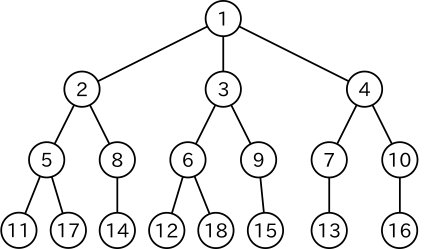
\includegraphics[width=.45\linewidth]
                    {initial-spanning-tree-18-example.pdf}
  }
  \caption{全域木初期グラフの例}
  \label{fig:initial-spanning-tree-example}
\end{figure}

定義\ref{def:stree-initial-graph}の初期グラフから探索することの
妥当性は証明されていない.次はその妥当性に関する予想である.
\begin{conjecture}\rm
  \label{conj:spanning-tree}
  一般化ムーアグラフ$M(n,k)$に,定義\ref{def:stree-initial-graph}
  で定義された全域木が存在する.
\end{conjecture}
また,条件を緩めて次も予想できる.
\begin{conjecture}\rm
  \label{conj:spanning-tree-2}
  一般化ムーアグラフ$M(n,k)$の全域木に,次の条件を満たす全域木が存在する.\par
  ある頂点$v$との距離が$Q$である頂点の集合$V=\{w\,|\,d(v,w)=Q\}$に
  ついて,次が成り立つ.
  \[ \max\{d(w)\,|\,w\in V\}-\min\{d(w)\,|\,w\in V\}\leq 1 \]
  つまり,次数の差がたかだか$1$である.
\end{conjecture}

初期グラフの変更を第\ref{chap:basic-algorithm}章で提案した方法に適応するには,
アルゴリズム\ref{algo:basic-algorithm}の2行目の$G_I$を新たに定義した
初期グラフに変更する.

\section{枝刈りによる探索空間の削減}
\label{sect:reduce-by-prune}
枝刈りによって探索空間を削減する.
本研究では,直径の下界を計算し,定理\ref{thm:gmg-geometric-property}
の条件(\ref{gmg-geom-b})を満足するか判断することで実現する.
直径の下界を計算する方法を与えるため,次のグラフを定義する.
\begin{definition}\rm
  探索途中の状態$(G,i)$に対するオペレータの適応を行う前とする.
  この状態について,グラフ$G$に候補辺番号$i$と$i$以降のすべての辺
  を追加したグラフを\textbf{最大グラフ}と定義する.
  このとき,最大グラフのもとになったグラフ$G$を\textbf{最小グラフ}と呼ぶ.
\end{definition}
\begin{example}\rm
  図\ref{fig:min-max-graph}に最小グラフと最大グラフの例を示す.
  図\ref{fig:min-graph-example}の破線部分はオペレータ適応の判定が行われていない候補辺を表す.
  最大グラフは,最小グラフのオペレータ適応未決定の辺をすべて追加したグラフと
  なっている.
\end{example}
\begin{figure}
  \centering
  \subfloat[最小グラフ(破線部分は未適応の候補辺)]{
    \includegraphics[width=.4\linewidth]
                    {min-graph-example.pdf}
    \label{fig:min-graph-example}
  }\hfill
  \subfloat[最大グラフ]{
    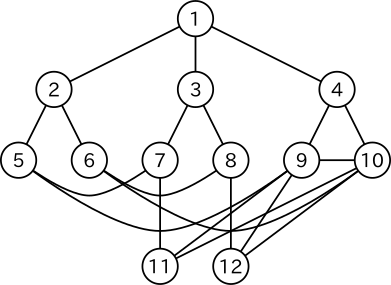
\includegraphics[width=.4\linewidth]
                    {max-graph-example.pdf}
    \label{fig:max-graph-example}
  }
  \caption{最小グラフと最大グラフの例}
  \label{fig:min-max-graph}
\end{figure}
直径の下界は,最大グラフの直径を計算すればよい.もし直径の下界が
定理\ref{thm:gmg-geometric-property}の条件(\ref{gmg-geom-b})を
満たさない場合,それ以降どのように辺を追加しても条件を満たさないので,
その場で探索を打ちきることができる.
この事実を応用して,一般化ムーアグラフの探索に直径の条件を考慮した
枝刈りをの方法を与える.探索で用いる状態は,最小グラフと最大グラフと候補辺の番号の
三つ組である.

次に,追加オペレータと無追加オペレータを新たに定めた状態に適応する.
追加オペレータは,最小グラフ$G_{\min}$と最大グラフ$G_{\max}$と候補辺番号$i$に
対して,最小グラフ$G'_{\min}=G_{\min}+e_i$と最大グラフ$G'_{\max}=G_{\max}$と
次の候補辺番号$i+1$を返す.また,無追加オペレータは,最小グラフ$G_{\min}$と
最大グラフ$G_{\max}$と候補辺番号$i$に対して,最小グラフ$G'_{\min}=G_{\min}$と
最大グラフ$G'_{\max}=G_{\max}-e_i$と次の候補辺番号$i+1$を返す.
さらに,系\ref{coll:basic-noadd-operator}で示した無追加オペレータの適応条件は
次のようになる.
\begin{corollary-without-proof}
  \label{coll:minmax-noadd-operator}
  \rm
  無追加オペレータについて,与えられた最小グラフを$G_{\min}$,最大グラフを
  $G_{\max}$,候補辺番号を$i$,対象の辺を$e_i=\{v,w\}$とし,
  適応後の最小グラフを$G'_{\min}$,最大グラフを$G'_{\max}$とする.
  $i$以降の辺の選び方次第で$G_{\min}'$が一般化ムーアグラフとなる見込み
  があることとは,次の二条件の両方を満たすことである.
  \begin{enumerate}
  \item 次数条件$\cdots$ $\text{Exit}(x)=i$なる$x\in e_i$について,
    $d_{G'_{\min}}(x)=k$.
  \item 直径条件$\cdots$ $G'_{\max}$の直径が定理\ref{thm:gmg-geometric-property}で
    示された直径以下である.
  \end{enumerate}
\end{corollary-without-proof}

本節で提案した枝刈りを第\ref{chap:basic-algorithm}章に示した方法に適応するには,
アルゴリズム\ref{algo:basic-algorithm}を次のように変更する.
\begin{itemize}
\item 4行目\ :\ $Stack\gets((G_I,G_I+\{e_i\}^M_{i\in\mathbb{N}},1))$
\item 6行目\ :\ $G,G_{\max},i\gets pop(Stack)$
\item 11行目\ :\ $operator$が$(G,G_{\max},i)$に適応できる
\item 12行目\ :\ $push(Stack,operator(G,G_{\max},i))$
\end{itemize}
さらに,各オペレータを本節で定義したものに変更する.

